\section{Multizbiory}

\textbf{Suma} -- $ \{ x \in U: x \in A \ \lor \ x \in B \} $

$$ A \cup B = \{ \ (x,f_{A \cup B} (x)): x \in U \ \textrm{i} \ f_{A \cup B}(x)=\max(f_A(x), f_B(x)) \ \} $$

\textbf{Iloczyn} -- $ \{ x: x \in U \ \land \ x \in A \ \land \ x \in B \} $

$$ A \cap B = \{ \ (x,f_{A \cap B} (x)): x \in U \ \textrm{i} \ f_{A \cap B}(x)=\min(f_A(x), f_B(x)) \ \} $$

\textbf{Różnica} -- $ \{ x: x \in U \ \land \ x \in A \ \land \ x \notin B \} $

$$ A \backslash B = \{ (x, f_{A \backslash B}(x)): x \in U \ \textrm{i} \ f_{A \backslash B}(x) = \textrm{min}(f_a(x), 1 - f_b(x)) \} $$

\textbf{Dopełnienie} -- $ \{ x \in U: x \notin A \} $

$$ - A = \{ (x, f_{-A}(x)): x \in U \ \textrm{i} \ f_{-A}(x) = 1 - f_{A}(x) \} $$

\textbf{Różnica symetryczna} -- $ \{ x: x \in U \ \land \ (x \in A \ \land \ x \notin B) \ \lor \ (x \in B \ \land \ x \notin A) \} $

$$ A \div B = \{ (x, f_{A \div B}(x)): x \in U \ \textrm{i} \ \max(\min(f_A(x), 1-f_B(x)), \min(f_B(x), 1-f_A(x))) \} $$ \medskip

$ X \subseteq Y $ - zawieranie, zbiór $X$ zawiera się lub jest równy zbiorowi $Y$.
Dosłownie każdy element $X$ jest w $Y$.

$ X \subset Y $ - zawieranie właściwe, zbiór $X$ zawiera się w $Y$ oraz $Y$ posiada jakiś element
który nie należy do $X$.

Dla dowolnych zbiorów $A, B, C$:
\begin{itemize}
    \item $\emptyset \subseteq A$
    \item jeżeli $ A \subseteq B $ i $ B \subseteq C $, to $ A \subseteq C $
\end{itemize}

\subsection{Zbiór potęgowy}
Przykład
$$ 2^{\{1, 2, 3\}} = \{\emptyset, \{1\}, \{2\}, \{3\}, \{1,2\}, \{1,3\}, \{2,3\}, \{1,2,3\}\} $$
$$ 2^{\emptyset} = \{ \emptyset \} $$

\subsection{Multizbiór}

\begin{center}
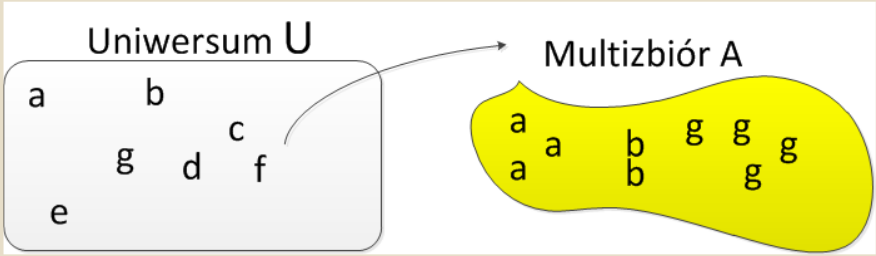
\includegraphics[scale=0.5]{img/multizbior.png}
\end{center}

$$ U = \{a, b, c, d, e, f, g\} \quad A=\{a, a, a, b, b, g, g, g, g\} $$

\begin{table}[!ht]
    \centering
    \caption{Funkcja charakterystyczna multizbioru $ f_a : U \to \{0, 1, ...\} $}
    \begin{adjustbox}{width=0.5\textwidth}
    \begin{tabular}{|c|c|c|c|c|c|c|c|}
        \hline
        x & a & b & c & d & e & f & g \\ \hline
        $f_a(x)$ & 3 & 2 & 0 & 0 & 0 & 0 & 4 \\ \hline
    \end{tabular}
\end{adjustbox}
\end{table}
$$ A=\{(x,fA(x)): x\in U\} \quad A= \{(a,3), (b,2), (c,0), (d,0), (e,0), (f,0), (g,4)\} $$ 

Nierozstrzygalne są : $ A \backslash B $ \ oraz \ $ A' $ (czyli dopełnienie).

\textbf{Przykład}

$ A=\{\ (a,3), (b,2), (c,0), (d,0), (e,4)\} = \{3a,2b,4e\ \} $

$ B=\{\ (a,0), (b,3), (c,1), (d,2), (e,0)\} = \{3b,c,2d\ \} $ \\

$ A \cap B = \{ \ (a,min(3,0)), (b,min(2,3)), (c,min(0,1)), (d,min(0,2)), (e,min(4,0))\} \\ = \{ \ (a,0),(b,2), (c,0), (d,0), (e,0) \ \} $ \\

$ A \cup B = \{ \ (a,3), (b,3), (c,1), (d,2), (e,4) \ \} $